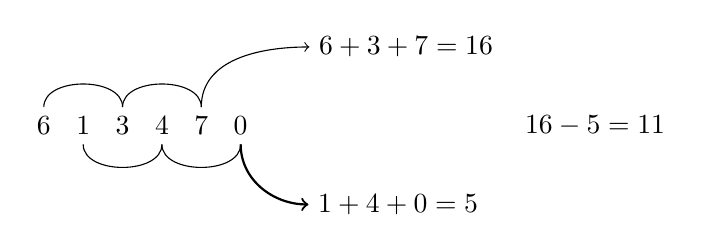
\begin{tikzpicture}
\node[] (A) at (0,0) {6};
\node[] (B) at (0.5,0) {1};
\node[] (C) at (1,0) {3};
\node[] (D) at (1.5,0) {4};
\node[] (E) at (2,0) {7};
\node[] (F) at (2.5,0) {0};

\node[] (I) at (4.6,1) {$6+3+7=16$} ;
\node[] (P) at (4.5,-1) {$1+4+0=5$} ;

\node[] (R) at (7,0) {$16-5=11$};

\draw[] (A)to[out=90,in=90](C);
\draw[] (C)to[out=90,in=90](E);
\draw[] (B)to[out=-90,in=-90](D);
\draw[] (D)to[out=-90,in=-90](F);
\draw[->] (E)to[out=90,in=180](I) ;
\draw[thick, ->] (F)to[out=-90,in=180](P);
\end{tikzpicture}
